% !TEX encoding = UTF-8
% !TEX TS-program = pdflatex
% !TEX root = ../tesi.tex

%**************************************************************
\chapter{Spring Cloud}\label{cap:spring-cloud}
%**************************************************************

%\epigraph{Citazione}{Autore della citazione}

\intro{Spring Cloud è un \textit{framework} del team Pivotal che offre gli strumenti necessari agli sviluppatori per implementare alcuni dei \textit{pattern} più comuni per i sistemi distribuiti,
quali ad esempio \textit{Service Discovery}, \textit{Circuit Breaker} e \textit{Intelligent Routing} (\textit{API Gateway}).}

\bigskip

Coordinare sistemi distribuiti basati su microservizi porta notoriamente a cosiddetti \textit{boiler plate practices}. \textit{Spring Cloud} subentra offrendo dei meccanismi che implementano le pratiche comuni, per fornire robustezza e automazione nella gestione dei sistemi distribuiti.

\clearpage

%--------------------------------------------------------------------------------------

\section{Spring Cloud Config}

\textit{Spring Cloud Config} è il modulo con il compito di gestire le configurazioni del sistema distribuito: copre il ruolo di \textit{Configuration Management}.
Viene fornita la possibilità di configurare sia il \textit{client side} che il \textit{server side}.

\subsection{Configurazioni lato client} Le configurazioni \textit{client side} si effettuano tramite
il file \texttt{bootstrap.properties}. Ad esempio, per configurare il nome dell'applicazione, si deve
modificare la proprietà \texttt{spring.application.name}, aggiungendo al file sopracitato il rigo:

\begin{tcolorbox}
\texttt{spring.application.name: myapp}
\end{tcolorbox}\addcontentsline{codes}{section}{Cambio nome applicazione (Spring)}

Le configurazioni \texttt{bootstrap} sono mostrate all'\textit{endpoint} \texttt{/env}, come mostrato nell'esempio che segue, assumendo che il servizio sia locato all'indirizzo \texttt{http://localhost:8080}:

\begin{tcolorbox}
	\begin{verbatim}
		$ curl localhost:8080/env
		{
		"profiles":[],
		"configService:https://github.com/spring-samples/
		config-repo/bar.properties":{"foo":"bar"},
		"servletContextInitParams":{},
		"systemProperties":{...},
		...
		}
	\end{verbatim}
\end{tcolorbox}\addcontentsline{codes}{section}{Esempio Spring Cloud client side configuration}

\subsection{Configurazioni lato server} Per abilitare la configurazione lato server, va usata l'annotazione \texttt{@EnableConfigServer}, come nello \textit{snippet} che segue:

\begin{tcolorbox}
	\begin{lstlisting}
@SpringBootApplication
@EnableConfigServer
public class ConfigServer {
  public static void main(String[] args) {
    SpringApplication.run(ConfigServer.class, args);
  }
}
	\end{lstlisting}
\end{tcolorbox}\addcontentsline{codes}{section}{Attivazione server side configuration (Spring Cloud)}

La strategia che governa la configurazione lato server è \texttt{EnvironmentRepository}, che serve oggetti \texttt{Environment}.

Le risorse \texttt{Environment} sono parametrizzate da tre variabili:
\begin{itemize}
	\item \texttt{\{application\}}: mappa \texttt{spring.application.name} del lato client;
	\item \texttt{\{profile\}}: mappa \texttt{spring.profiles.active} del lato client, che indica il profilo attivo (sviluppo, produzione, etc\dots);
	\item \texttt{\{label\}}: etichetta un insieme di file di configurazione.
\end{itemize}

Come default, \texttt{EnvironmentRepository} usa come \textit{backend} il sistema di controllo versione \textit{Git}.
La proprietà \texttt{spring.cloud.config.server.git.uri} può essere impostata per cambiare l'URL della repository di \textit{back-end}.
Può puntare sia a una \textit{repository} remota (tramite prefissi \texttt{http:}, \texttt{https:}, etc\dots) che una locale (tramite il prefisso \texttt{file:}).

Tramite \textit{Cloud Config} è possibile fare una miriade di altre configurazioni, tra cui:

\begin{itemize}
	\item Disabilitare la validazione tramite certificato SSL;
	\item Impostare un \textit{timeout} per la connessione HTTP;
	\item Supportare multiple \textit{repository};
	\item Supportare l'autenticazione.
\end{itemize}

\subsection{Health indicator} \textit{Cloud Config} supporta nativamente un indicatore che
tiene sotto controllo lo stato dell'\texttt{Environment Repository} configurata.
È possibile disabilitare tale indicatore impostando la proprietà \texttt{spring.cloud.config.server.health.enabled} a falso.

\bigskip

\textit{Spring Cloud Config} offre molte altre opzioni e funzionalità che non verranno ulteriormente approfondite, poiché lo scopo di questa appendice è quello di dare una semplice infarinatura sul \textit{framework}.

%--------------------------------------------------------------------------------------

\section{Service Discovery con Netflix Eureka}

Per implementare il pattern \textit{Service Discovery} (discusso in \S\ref{service-discovery}) e molti altri, Spring si appoggia a \textit{Netflix Open Source Software} (\textit{Netflix OSS}), una raccolta di librerie offerte da Netflix.
Integra \textit{Netflix Eureka} come servizio con ruolo di \textit{Service Discovery}, lato client e server. \textit{Spring Cloud} offre diverse alternative per i vari pattern, tuttavia ne verranno discussi solo alcuni.

\begin{figure}[H]
	\centering
	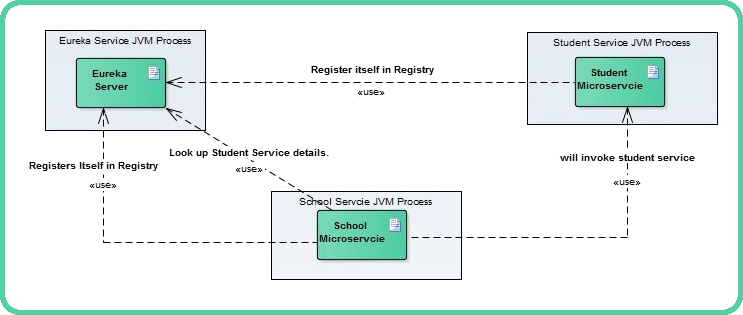
\includegraphics[width=\textwidth]{immagini/netflix-eureka.png}
	\caption[Spring Cloud Service Discovery con Netflix Eureka]{Spring Cloud Service Discovery con Netflix Eureka\footnotemark}
	\label{netflix-eureka}
\end{figure}
\footnotetext{Fonte immagine: \href{https://howtodoinjava.com/spring-cloud/spring-cloud-service-discovery-netflix-eureka/}{https://howtodoinjava.com}}

Vedendo \ref{netflix-eureka}, è possibile notare che ogni \textit{client} può registrarsi a \texttt{Eureka Server}, fornendo meta-dati di sé stesso, tra cui \textit{host}, porta, URL dell'\textit{Health Indicator}, \textit{home page}, e altri dettagli.

\subsection{Uso di EurekaClient} Una volta che un'applicazione è registrata nel \textit{Service Discovery} di \textit{Eureka}, è possibile utilizzare \texttt{EurekaClient} per scoprire i servizi che sono registrati, come mostrato nell'esempio seguente:

 \begin{tcolorbox}
 	\begin{lstlisting}
@Autowired
private EurekaClient discoveryClient;

public String serviceUrl() {
  InstanceInfo instance = discoveryClient.getNextServerFromEureka("STORES", false);
  return instance.getHomePageUrl();
}
 	\end{lstlisting}
 \end{tcolorbox}\addcontentsline{codes}{section}{Discover dei servizi registrati su EurekaServer}

\texttt{@Autowired} è un'annotazione che permette di iniettare i cosiddetti \textit{bean} di \textit{Spring} tramite \textit{dependency injection}. Nella variabile \texttt{instance} saranno salvate le informazioni relative al servizio di interesse.

\subsection{EurekaServer} Per utilizzare un applicazione come \texttt{EurekaServer}, è sufficiente utilizzare l'annotazione \texttt{@EnableEurekaServer} nella classe contenente il \textit{main}.

%--------------------------------------------------------------------------------------

\section{Circuit Breaker con Netflix Hystrix}

\textit{Netflix} offre una libreria che implementa il \textit{Circuit Breaker pattern}, già discusso in \S\ref{circuit-breaker}: \textit{Hystrix}.

È possibile vedere l'interfaccia del servizio nella figura che segue:

\begin{figure}[H]
	\centering
	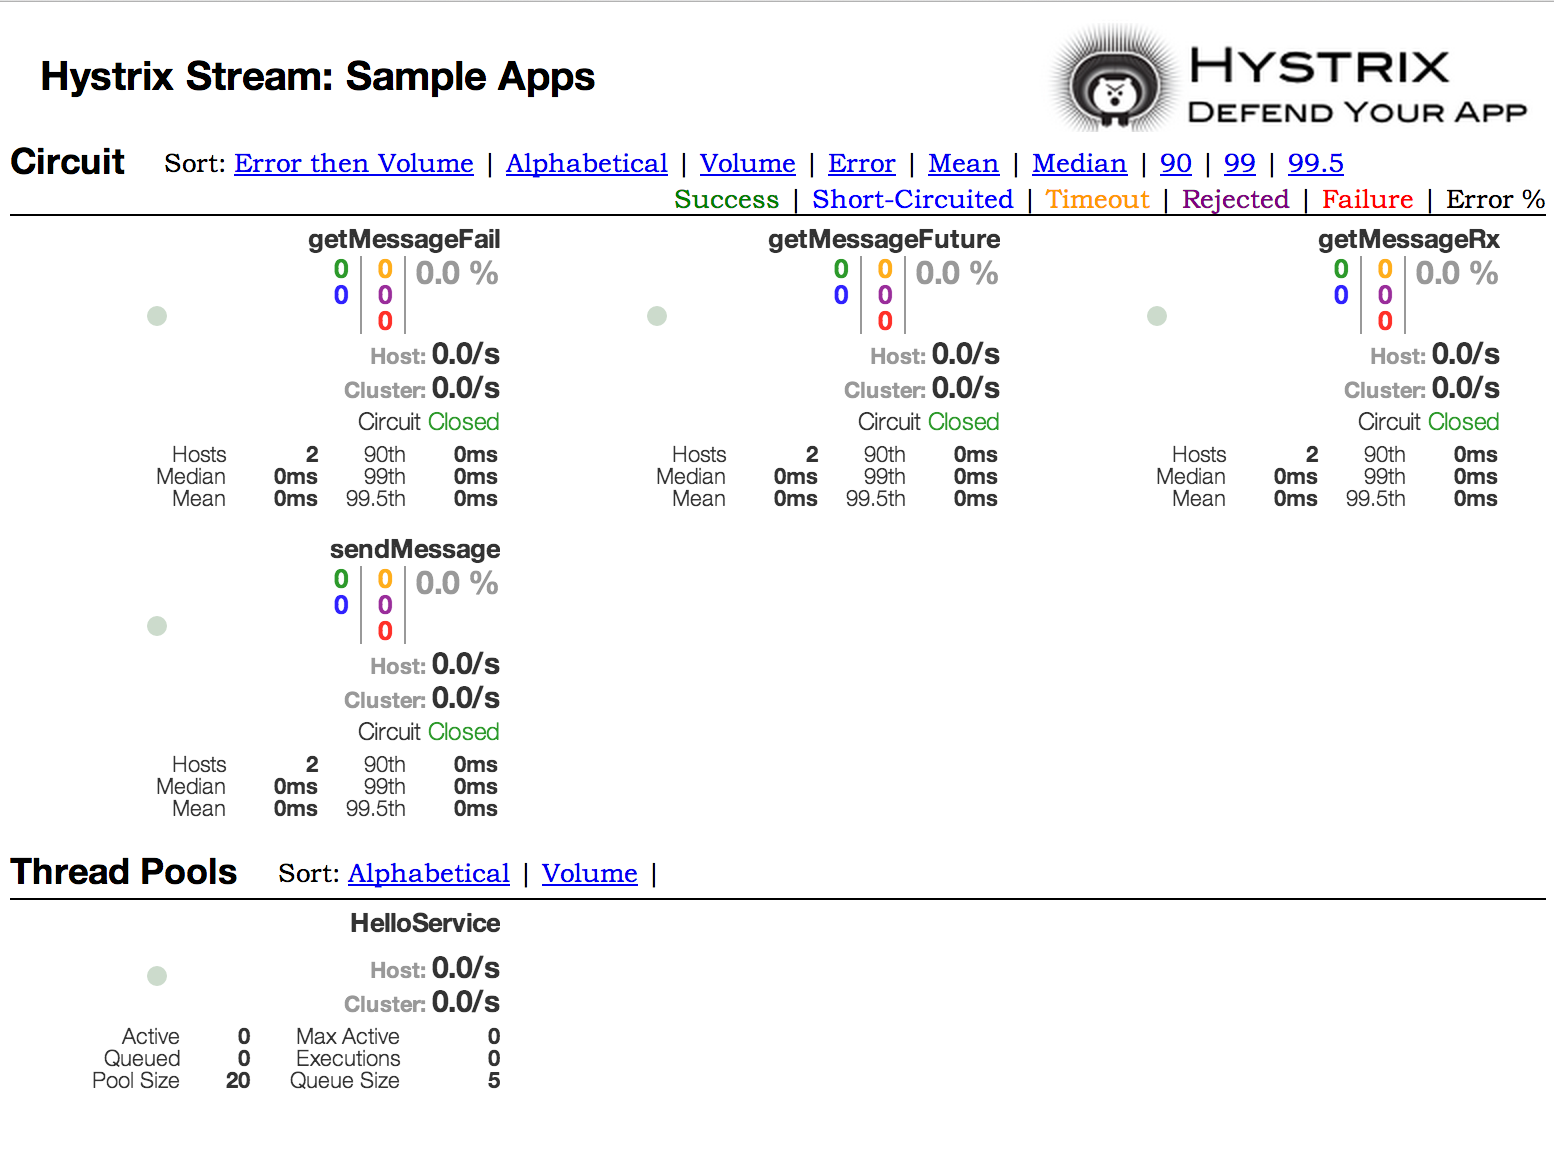
\includegraphics[width=\textwidth]{immagini/Hystrix.png}
	\caption[Interfaccia di Netflix Hystrix]{Interfaccia di Netflix Hystrix\footnotemark}
	\label{netflix-hystrix}
\end{figure}
\footnotetext{Fonte immagine: \href{https://cloud.spring.io/spring-cloud-static/Greenwich.SR1/single/spring-cloud.html}{https://cloud.spring.io}}

\textit{Spring Cloud} usa \textit{Hystrix} come \textit{Circuit Breaker}:
quando una chiamata a un particolare servizio eccede la proprietà \texttt{requestVolumeThreshold} (il valore di default è 20 richieste) e la percentuale di fallimento è maggiore di \texttt{errorThresholdPercentage} (default 50\%) in una finestra di tempo limitato,
il \textit{Circuit Breaker} si apre e le chiamate vengono prevenute e sostituite da chiamate di \textit{fallback} definite nel circuito.

\subsection{Abilitare Hystrix} Per abilitare \textit{Hystrix} in un'applicazione \textit{Spring},
è sufficiente usare l'annotazione \texttt{@EnableCircuitBreaker} nella classe contenente il \textit{main}.

Segue un minimale esempio d'uso di \textit{Hystrix}:


\begin{tcolorbox}
	\begin{lstlisting}
@Component
public class StoreIntegration {

  @HystrixCommand(fallbackMethod = "defaultStores")
  public Object getStores(Map<String, Object> parameters) {
    //do stuff that might fail
  }

  public Object defaultStores(Map<String, Object> parameters) {
    return /* something useful */;
  }
}
	\end{lstlisting}
\end{tcolorbox}\addcontentsline{codes}{section}{Esempio di Circuit Breaker con Netflix Hystrix}

Viene definito il metodo \texttt{getStores()} che effettua della logica con una \texttt{Map} passata come parametro.
L'annotazione \texttt{@HystrixCommand} definisce una chiamata di \textit{callback} in caso di attivazione del \textit{Circuit Breaker} verso il metodo \texttt{defaultStores()}.


%--------------------------------------------------------------------------------------

\section{API Gateway con Netflix Zuul}

Il \textit{routing} è una parte essenziale di un'architettura a microservizi. Come esempio, \texttt{/} potrebbe essere mappato sulla \textit{web application}, \texttt{/api/users} sul servizio utenti e \texttt{/api/shop} sul servizio di shopping.

\textit{Zuul} è un \textit{router} e \textit{load balancer} lato server basato su \textit{Java Virtual Machine} rilasciato da \textit{Netflix}. \textit{Spring Cloud} lo integra come \textit{router} principale. In quanto gestore del routing dei vari microservizi, svolge il ruolo di \textit{API Gateway} (discusso in \S\ref{api-gateway})

\begin{figure}[H]
	\centering
	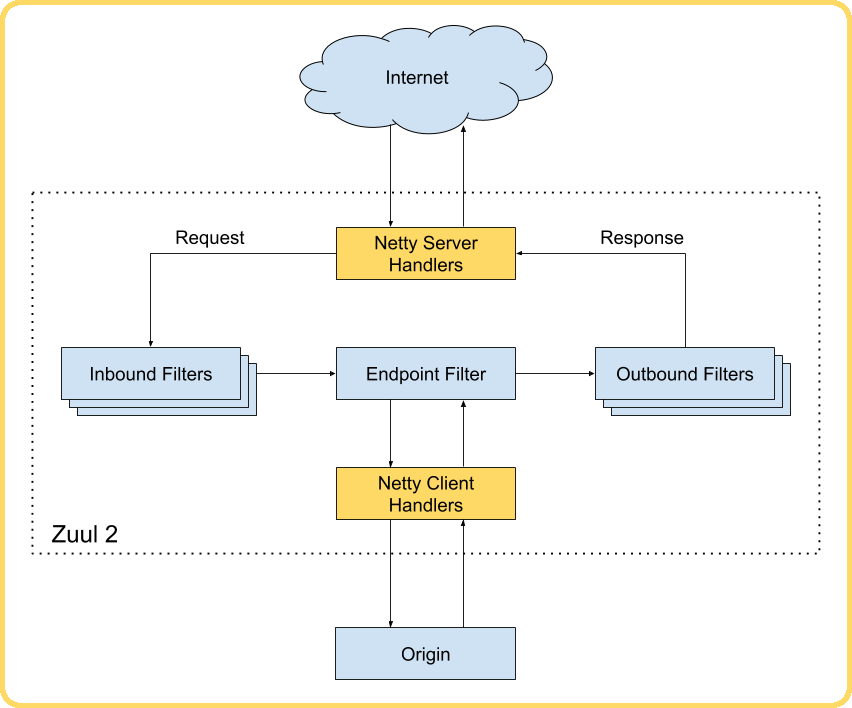
\includegraphics[width=\textwidth]{immagini/zuul.png}
	\caption[Panoramica di Netflix Zuul]{Panoramica di Netflix Zuul\footnotemark}
	\label{netflix-zuul}
\end{figure}
\footnotetext{Fonte immagine: \url{https://github.com/Netflix/zuul/wiki/How-It-Works-2.0}}

\subsection{Abilitare Zuul Reverse Proxy} Spring Cloud ha creato un \textit{proxy} integrato di \textit{Zuul} per aiutare lo sviluppo in casi d'uso comuni in cui un'applicazione UI voglia fare delle chiamate \textit{proxy} a uno o più servizi di \textit{back-end}, chiamato \textit{Zuul Reverse Proxy}.

Per abilitare \textit{Zuul Reverse Proxy}, basta annotare la classe \textit{main} con \texttt{@EnableZuulProxy}.

Sotto la proprietà \texttt{zuul.routes} sono elencati tutti i servizi gestiti dal \textit{routing} di \textit{Zuul}.
Vediamo un esempio.

\begin{tcolorbox}
	\begin{verbatim}
		zuul.routes.users.path: /myusers/**
	\end{verbatim}
\end{tcolorbox}\addcontentsline{codes}{section}{Configurazione di routing con Netflix Zuul}

In questo caso, tutte le chiamate a \texttt{/myusers} sono mappate all'\textit{endpoint} \texttt{/myusers} del servizio \texttt{users}.

È possibile ignorare alcuni pattern con la proprietà \texttt{zuul.ignoredPatterns}, per ragioni di sicurezza o altro, come ad esempio:

\begin{tcolorbox}
	\begin{verbatim}
	zuul.ignoredPatterns: /**/admin/**
	\end{verbatim}
\end{tcolorbox}\addcontentsline{codes}{section}{Pattern ignorati da Zuul}

In questo caso, considerando anche la proprietà impostata nell'esempio precedente, tutte le chiamate a \texttt{/myusers} vengono mappate tali quali a prima, ad eccezione di quelle che includono il \textit{pattern} \texttt{/admin/}, le quali vengono rigettate.

\subsection{Endpoint di Zuul} \textit{Zuul} mette a disposizione due \textit{endpoint}:
\begin{itemize}
	\item \texttt{/routes};
	\item \texttt{/filters}.
\end{itemize}

Una chiamata GET all'endpoint \texttt{/routes} può risultare in una risposta similare:

\begin{tcolorbox}
	\begin{verbatim}
{
    "/stores/**": "http://localhost:8081"
}
	\end{verbatim}
\end{tcolorbox}\addcontentsline{codes}{section}{Zuul: GET /routes}

Vengono restituiti tutti i servizi gestiti dal \textit{routing} di \textit{Zuul}, con nome e indirizzo originale.

Attraverso \texttt{/filters} è possibile ottenere una mappa dei filtri di \textit{Zuul} divisi per tipo.

%--------------------------------------------------------------------------------------

\section{Spring Cloud Stream}

\textit{Spring Cloud Stream} è un modulo di \textit{Spring Cloud} che permette di connettere l'applicazione a un \textit{message broker},
ossia un gestore di code di messaggi (quali \textit{Apache Kafka} o \textit{RabbitMQ}).

Il modulo può essere visto comunemente come la ``fusione'' tra \textit{Spring Boot} e \textit{Spring Integration}.

\begin{figure}[H]
	\centering
	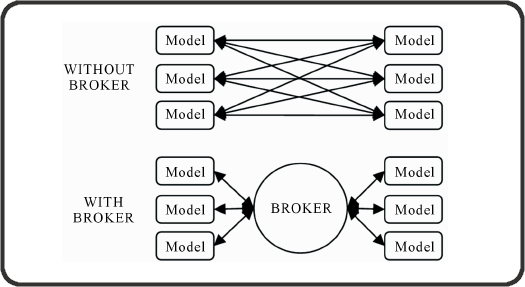
\includegraphics[width=\textwidth]{immagini/message-broker.png}
	\caption[Message broker]{Message broker\footnotemark}
	\label{message-broker}
\end{figure}
\footnotetext{Fonte immagine: \url{https://www.researchgate.net}}

L'uso di un \textit{broker} permette di rendere i microservizi tra loro asincroni e trasferire alcune responsabilità di \textit{business logic} alla gestione dei messaggi del \textit{broker} stesso.

Comunicando esclusivamente via HTTP non si avrebbe il vantaggio dell'asincronicità dei microservizi: cosa succederebbe se il \textit{client} A notificasse un evento di interesse del \textit{client} B, immaginando che quest'ultimo sia momentaneamente indisponibile?
In caso di servizi sincroni, il messaggio verrebbe perso. Avendo invece a disposizione una coda di messaggi, il \textit{client} B potrebbe recuperare il messaggio in qualsiasi momento, una volta tornato disponibile.

Vediamo un esempio d'uso di \textit{Spring Cloud Stream}.
\begin{tcolorbox}
	\begin{lstlisting}
@SpringBootApplication
@EnableBinding(Sink.class)
public class LoggingConsumerApplication {

  public static void main(String[] args) {
    SpringApplication.run(LoggingConsumerApplication.class, args);
  }

  @StreamListener(Sink.INPUT)
  public void handle(Person person) {
    System.out.println("Received: " + person);
  }
}
	\end{lstlisting}
\end{tcolorbox}\addcontentsline{codes}{section}{Uso di Spring Cloud Stream}

Abbiamo il metodo \texttt{handle()} che gestisce i messaggi in entrata per il tipo \texttt{Person}.
Qui entra in gioco il \textit{framework}: cerca di convertire automaticamente il messaggio (in formato JSON) nel tipo \texttt{Person} riconosciuto dall'applicazione, che potrà usarlo per qualsivoglia logica.

In questo caso, stampa semplicemente a video un messaggio che mostra la persona ricevuta e convertita dal messaggio.

\bigskip

\textit{Spring Cloud Stream} offre dei \textit{binder} sia per \textit{Apache Kafka} che per \textit{Rabbit MQ}.